% ------------------------------------------------------------
\chapter{Implementation}
\setlength{\parindent}{0pt}
\setlength{\parskip}{6pt}
{\setstretch{1.5}

This chapter describes the practical implementation of the \textbf{ResQNow} emergency response system through detailed pseudocode and actual code implementations. It explains how the core functionalities—SOS alert triggering, Bluetooth Low Energy (BLE) based offline communication, AI-driven emergency classification, and backend services—were developed and integrated. The chapter presents code-level evidence to demonstrate the working of critical system modules.

% -----------------------------------------------------------------------------
\section{SOS Activation and Emergency Alert Implementation}

The SOS module serves as the primary emergency trigger in ResQNow. It enables users to initiate emergency alerts manually or automatically based on AI classification. Upon activation, the system captures GPS location, timestamps the event, and initiates alert propagation through available communication channels.

\subsection{SOS Activation Pseudocode}

The following pseudocode outlines the SOS activation workflow:

\begin{algorithm}[H]
\caption{SOS Activation and Alert Dispatch}
\begin{algorithmic}[1]
\State \textbf{Input:} User trigger (button press or voice command)
\State \textbf{Output:} SOS alert dispatched to backend and emergency contacts
\State
\Procedure{ActivateSOS}{}
    \State $location \gets$ \Call{GetGPSLocation}{}
    \State $timestamp \gets$ \Call{GetCurrentTimestamp}{}
    \State $userId \gets$ \Call{GetAuthenticatedUserId}{}
    \State
    \State $sosData \gets$ \{
    \State \hspace{1cm} userId: $userId$,
    \State \hspace{1cm} latitude: $location.latitude$,
    \State \hspace{1cm} longitude: $location.longitude$,
    \State \hspace{1cm} timestamp: $timestamp$,
    \State \hspace{1cm} severity: "pending\_classification"
    \State \}
    \State
    \If{InternetAvailable()}
        \State \Call{SendSOSToBackend}{$sosData$}
        \State \Call{NotifyEmergencyContacts}{$sosData$}
    \Else
        \State \Call{QueueForBLERelay}{$sosData$}
        \State \Call{InitiateBLEBroadcast}{$sosData$}
    \EndIf
    \State
    \State \Call{DisplayConfirmation}{"SOS Alert Activated"}
\EndProcedure
\end{algorithmic}
\end{algorithm}

\subsection{SOS User Interface Implementation}

The SOS activation interface is implemented with minimal interaction requirements to ensure rapid activation during emergencies. Figure~\ref{fig:sos_ui} presents the user interface implementation showing the emergency trigger button and status display.

\begin{figure}[H]
    \centering
    \includegraphics[width=\textwidth]{chapters/sos_ui.png}
    \caption{SOS activation interface enabling rapid emergency alert triggering}
    \label{fig:sos_ui}
\end{figure}

\subsection{Backend SOS Handling Implementation}

The backend validates incoming SOS requests, stores emergency data in Firestore, triggers multi-channel notifications, and tracks responder acknowledgments. Figure~\ref{fig:sos_backend} illustrates the FastAPI implementation for handling SOS requests, including authentication validation, data persistence, and alert orchestration logic.

\begin{figure}[H]
    \centering
    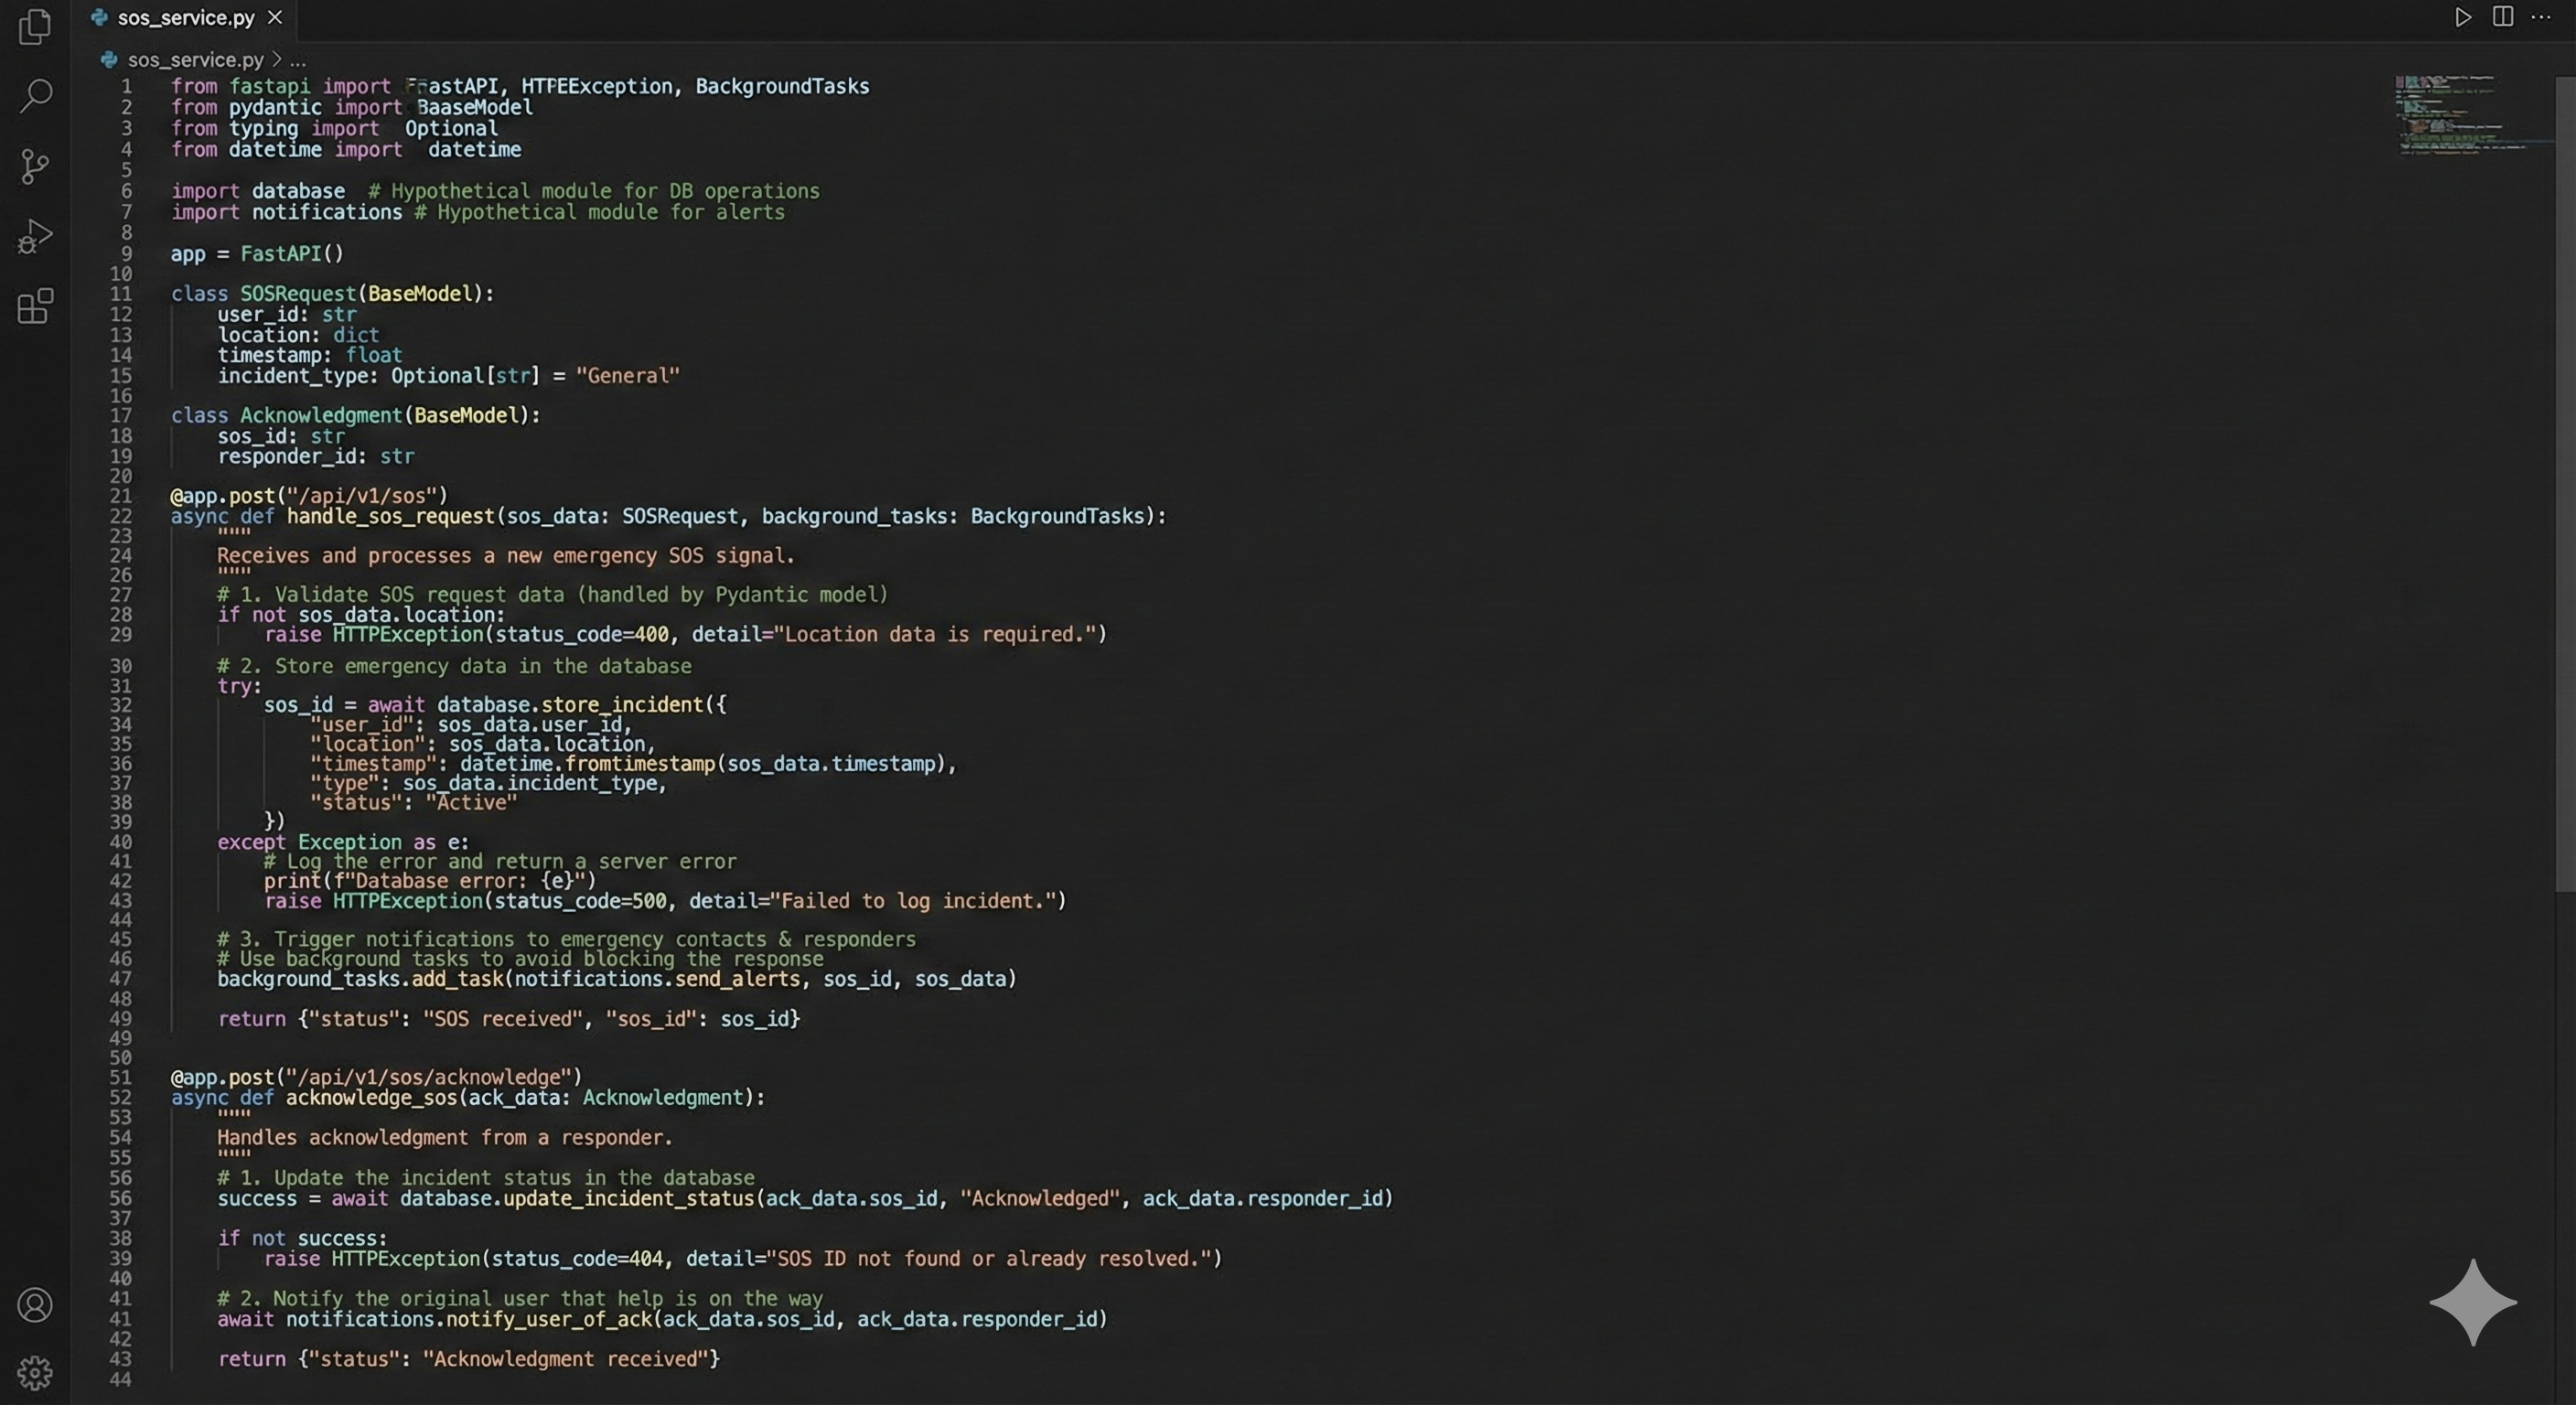
\includegraphics[width=0.9\textwidth]{chapters/sos_backend_code.png}
    \caption{Backend implementation for SOS request handling and alert orchestration}
    \label{fig:sos_backend}
\end{figure}

The backend implementation ensures reliable emergency alert coordination with proper error handling and logging mechanisms for system monitoring and debugging purposes.

% -----------------------------------------------------------------------------
\section{Bluetooth Low Energy (BLE) Offline Communication Implementation}

To support emergency alert delivery in low or no internet connectivity environments, ResQNow implements BLE-based offline SOS relay. The BLE communication module is optimized for low power consumption and dynamically discovers nearby devices running ResQNow to establish secure short-range connections.

\subsection{BLE Message Relay Pseudocode}

The following pseudocode describes the BLE offline relay mechanism:

\begin{algorithm}[H]
\caption{BLE Offline SOS Relay}
\begin{algorithmic}[1]
\State \textbf{Input:} SOS message to be relayed
\State \textbf{Output:} SOS delivered to device with internet connectivity
\State
\Procedure{InitiateBLERelay}{$sosMessage$}
    \State $encryptedMessage \gets$ \Call{EncryptAES}{$sosMessage$}
    \State $nearbyDevices \gets$ \Call{ScanForBLEDevices}{}
    \State
    \If{$nearbyDevices.length > 0$}
        \For{each $device$ in $nearbyDevices$}
            \State \Call{ConnectToDevice}{$device$}
            \State \Call{TransmitMessage}{$device$, $encryptedMessage$}
        \EndFor
    \Else
        \State \Call{QueueMessage}{$encryptedMessage$}
        \State \Call{RetryAfterDelay}{5 seconds}
    \EndIf
\EndProcedure
\State
\Procedure{ReceiveBLEMessage}{$encryptedMessage$, $sourceDevice$}
    \State $sosMessage \gets$ \Call{DecryptAES}{$encryptedMessage$}
    \State
    \If{InternetAvailable()}
        \State \Call{UploadSOSToBackend}{$sosMessage$}
        \State \Call{SendAcknowledgment}{$sourceDevice$}
    \Else
        \State \Call{RelayToOtherDevices}{$encryptedMessage$}
    \EndIf
\EndProcedure
\end{algorithmic}
\end{algorithm}

\subsection{BLE Relay Workflow Diagram}

The BLE module enables nearby ResQNow devices to form a temporary peer-to-peer relay network where encrypted SOS packets are forwarded hop-by-hop until a device with internet connectivity is reached. Figure~\ref{fig:ble_workflow} illustrates the complete BLE offline relay workflow, showing device discovery, message encryption, peer-to-peer transmission, and eventual upload to the backend server.

\begin{figure}[H]
    \centering
    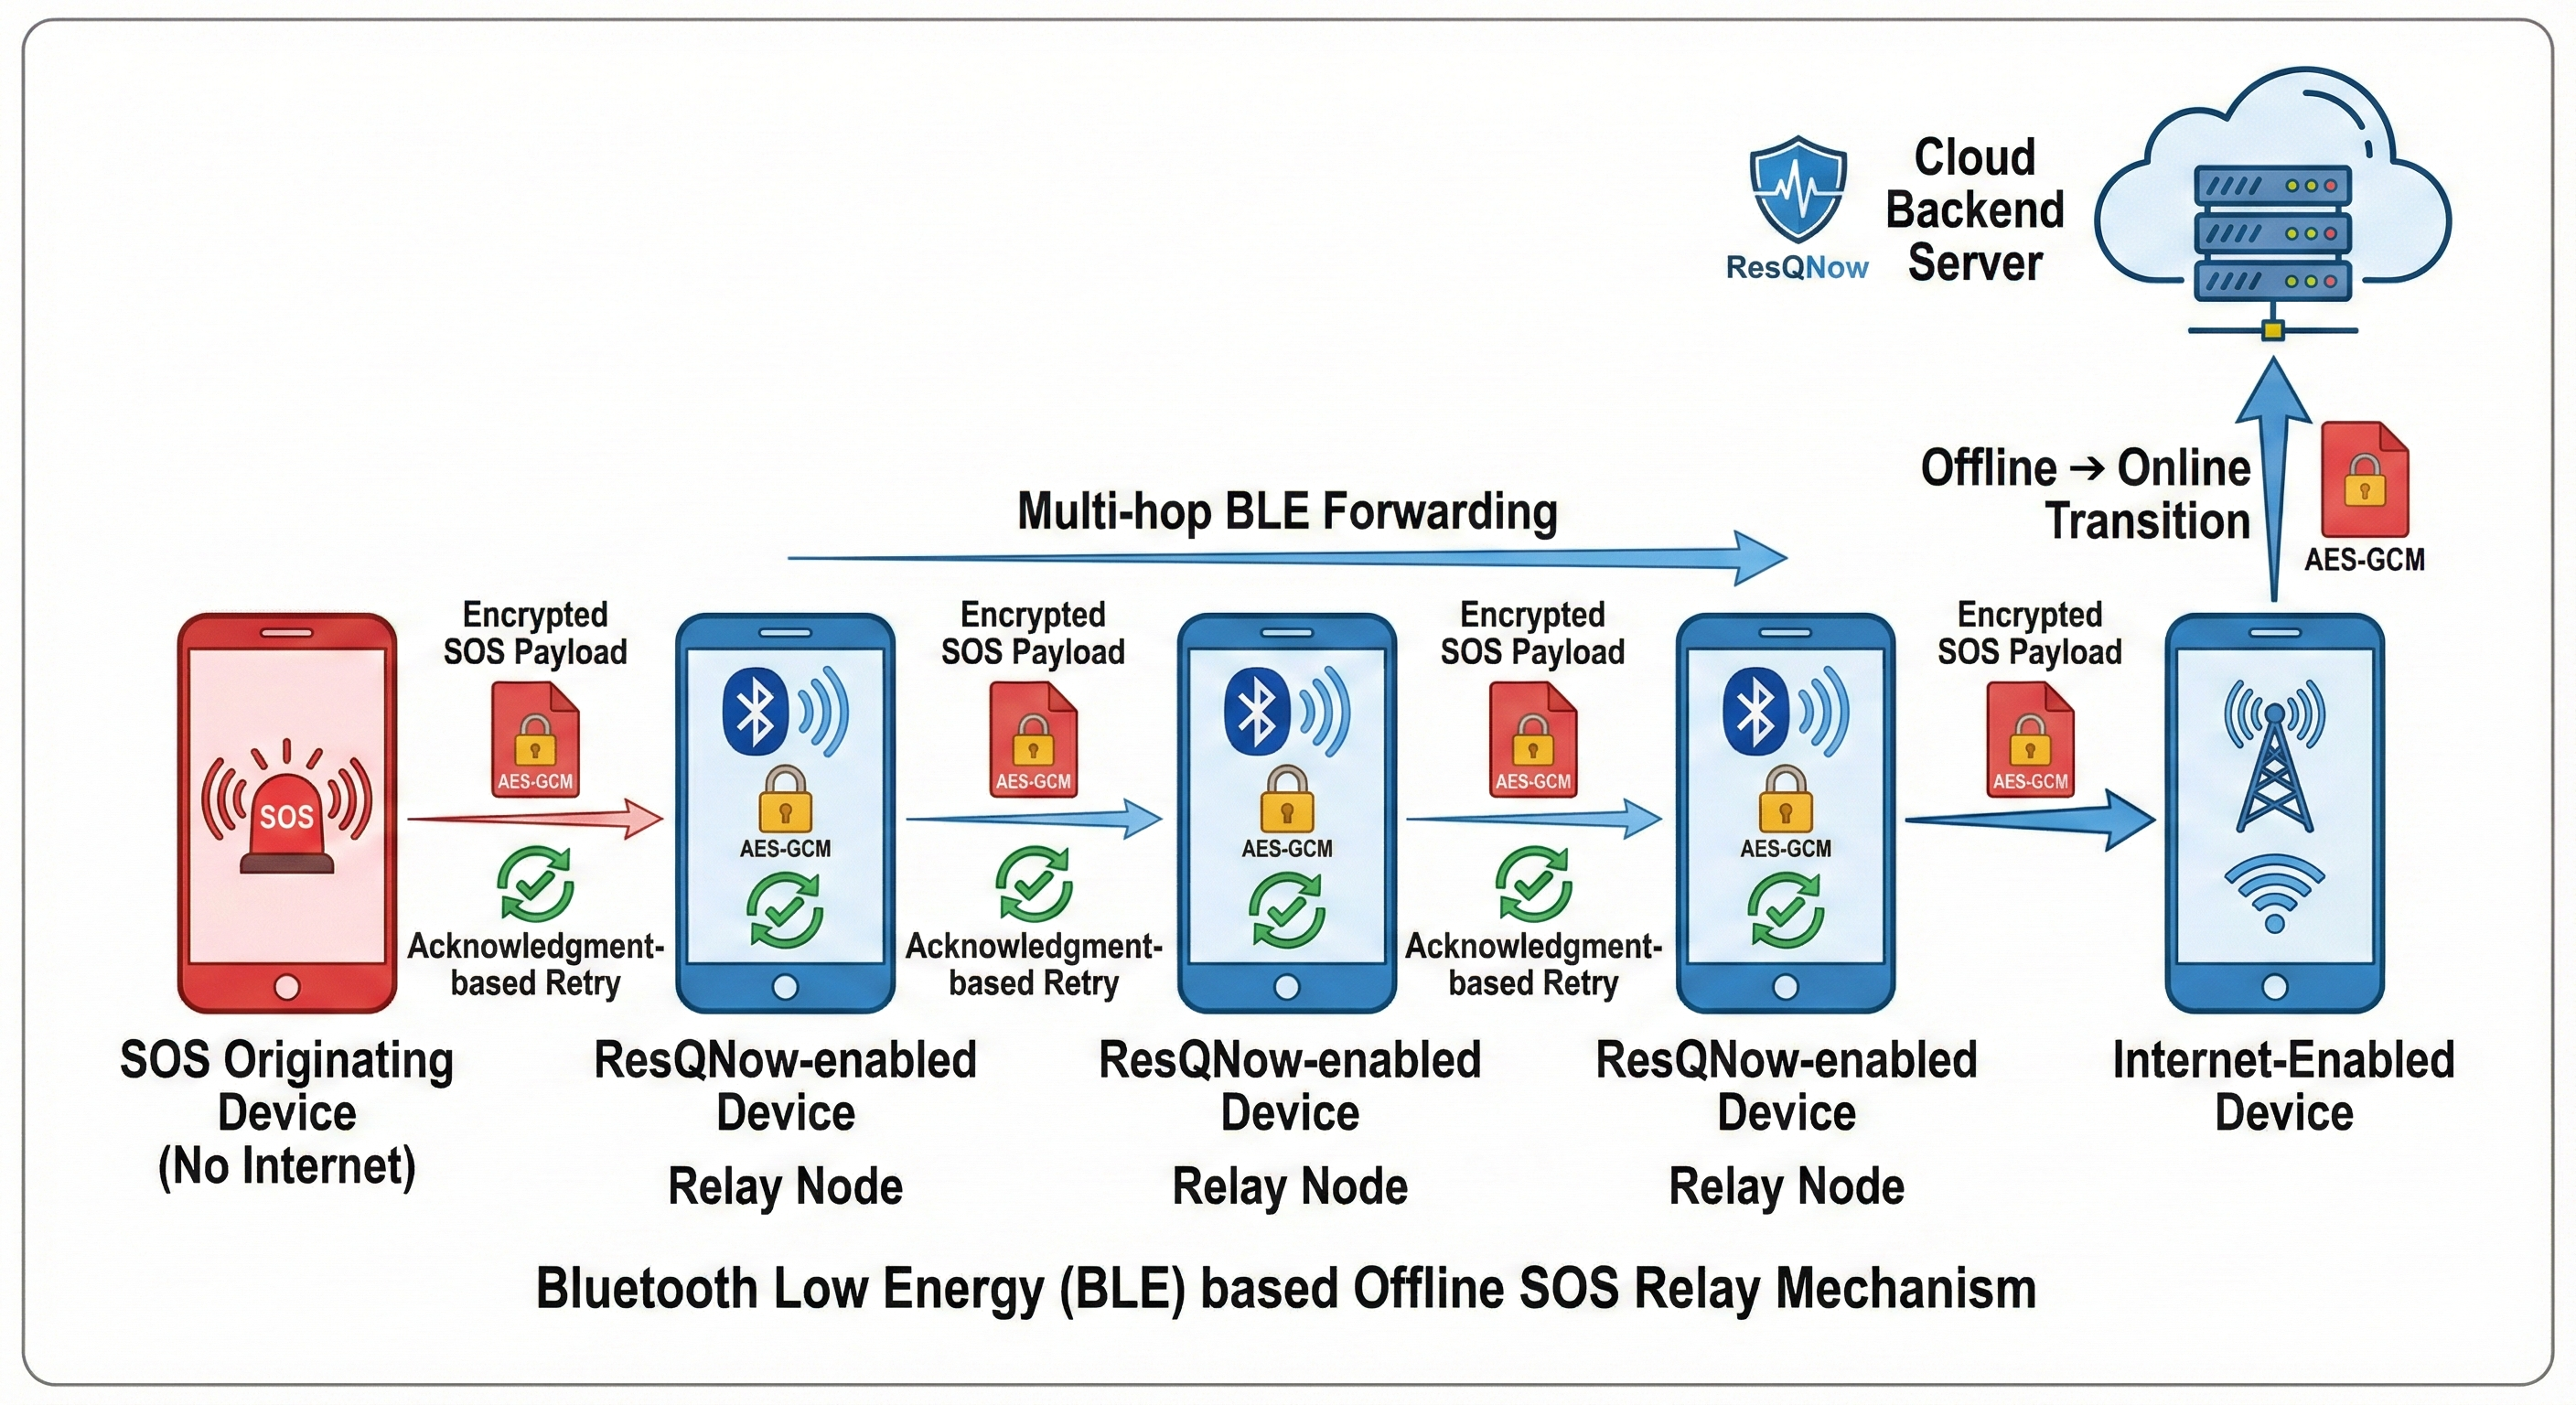
\includegraphics[width=0.9\textwidth]{chapters/ble_relay_workflow.png}
    \caption{BLE-based offline SOS relay mechanism across nearby devices}
    \label{fig:ble_workflow}
\end{figure}

\subsection{BLE Encryption and Transmission Code}

To protect sensitive emergency data during transmission, BLE messages are encrypted using AES-128 in GCM (Galois/Counter Mode) prior to wireless transmission. Figure~\ref{fig:ble_code} demonstrates the code-level implementation for encrypted BLE message transmission and reception, including key generation, message encryption, Bluetooth characteristic writing, and decryption upon receipt.

\begin{figure}[H]
    \centering
    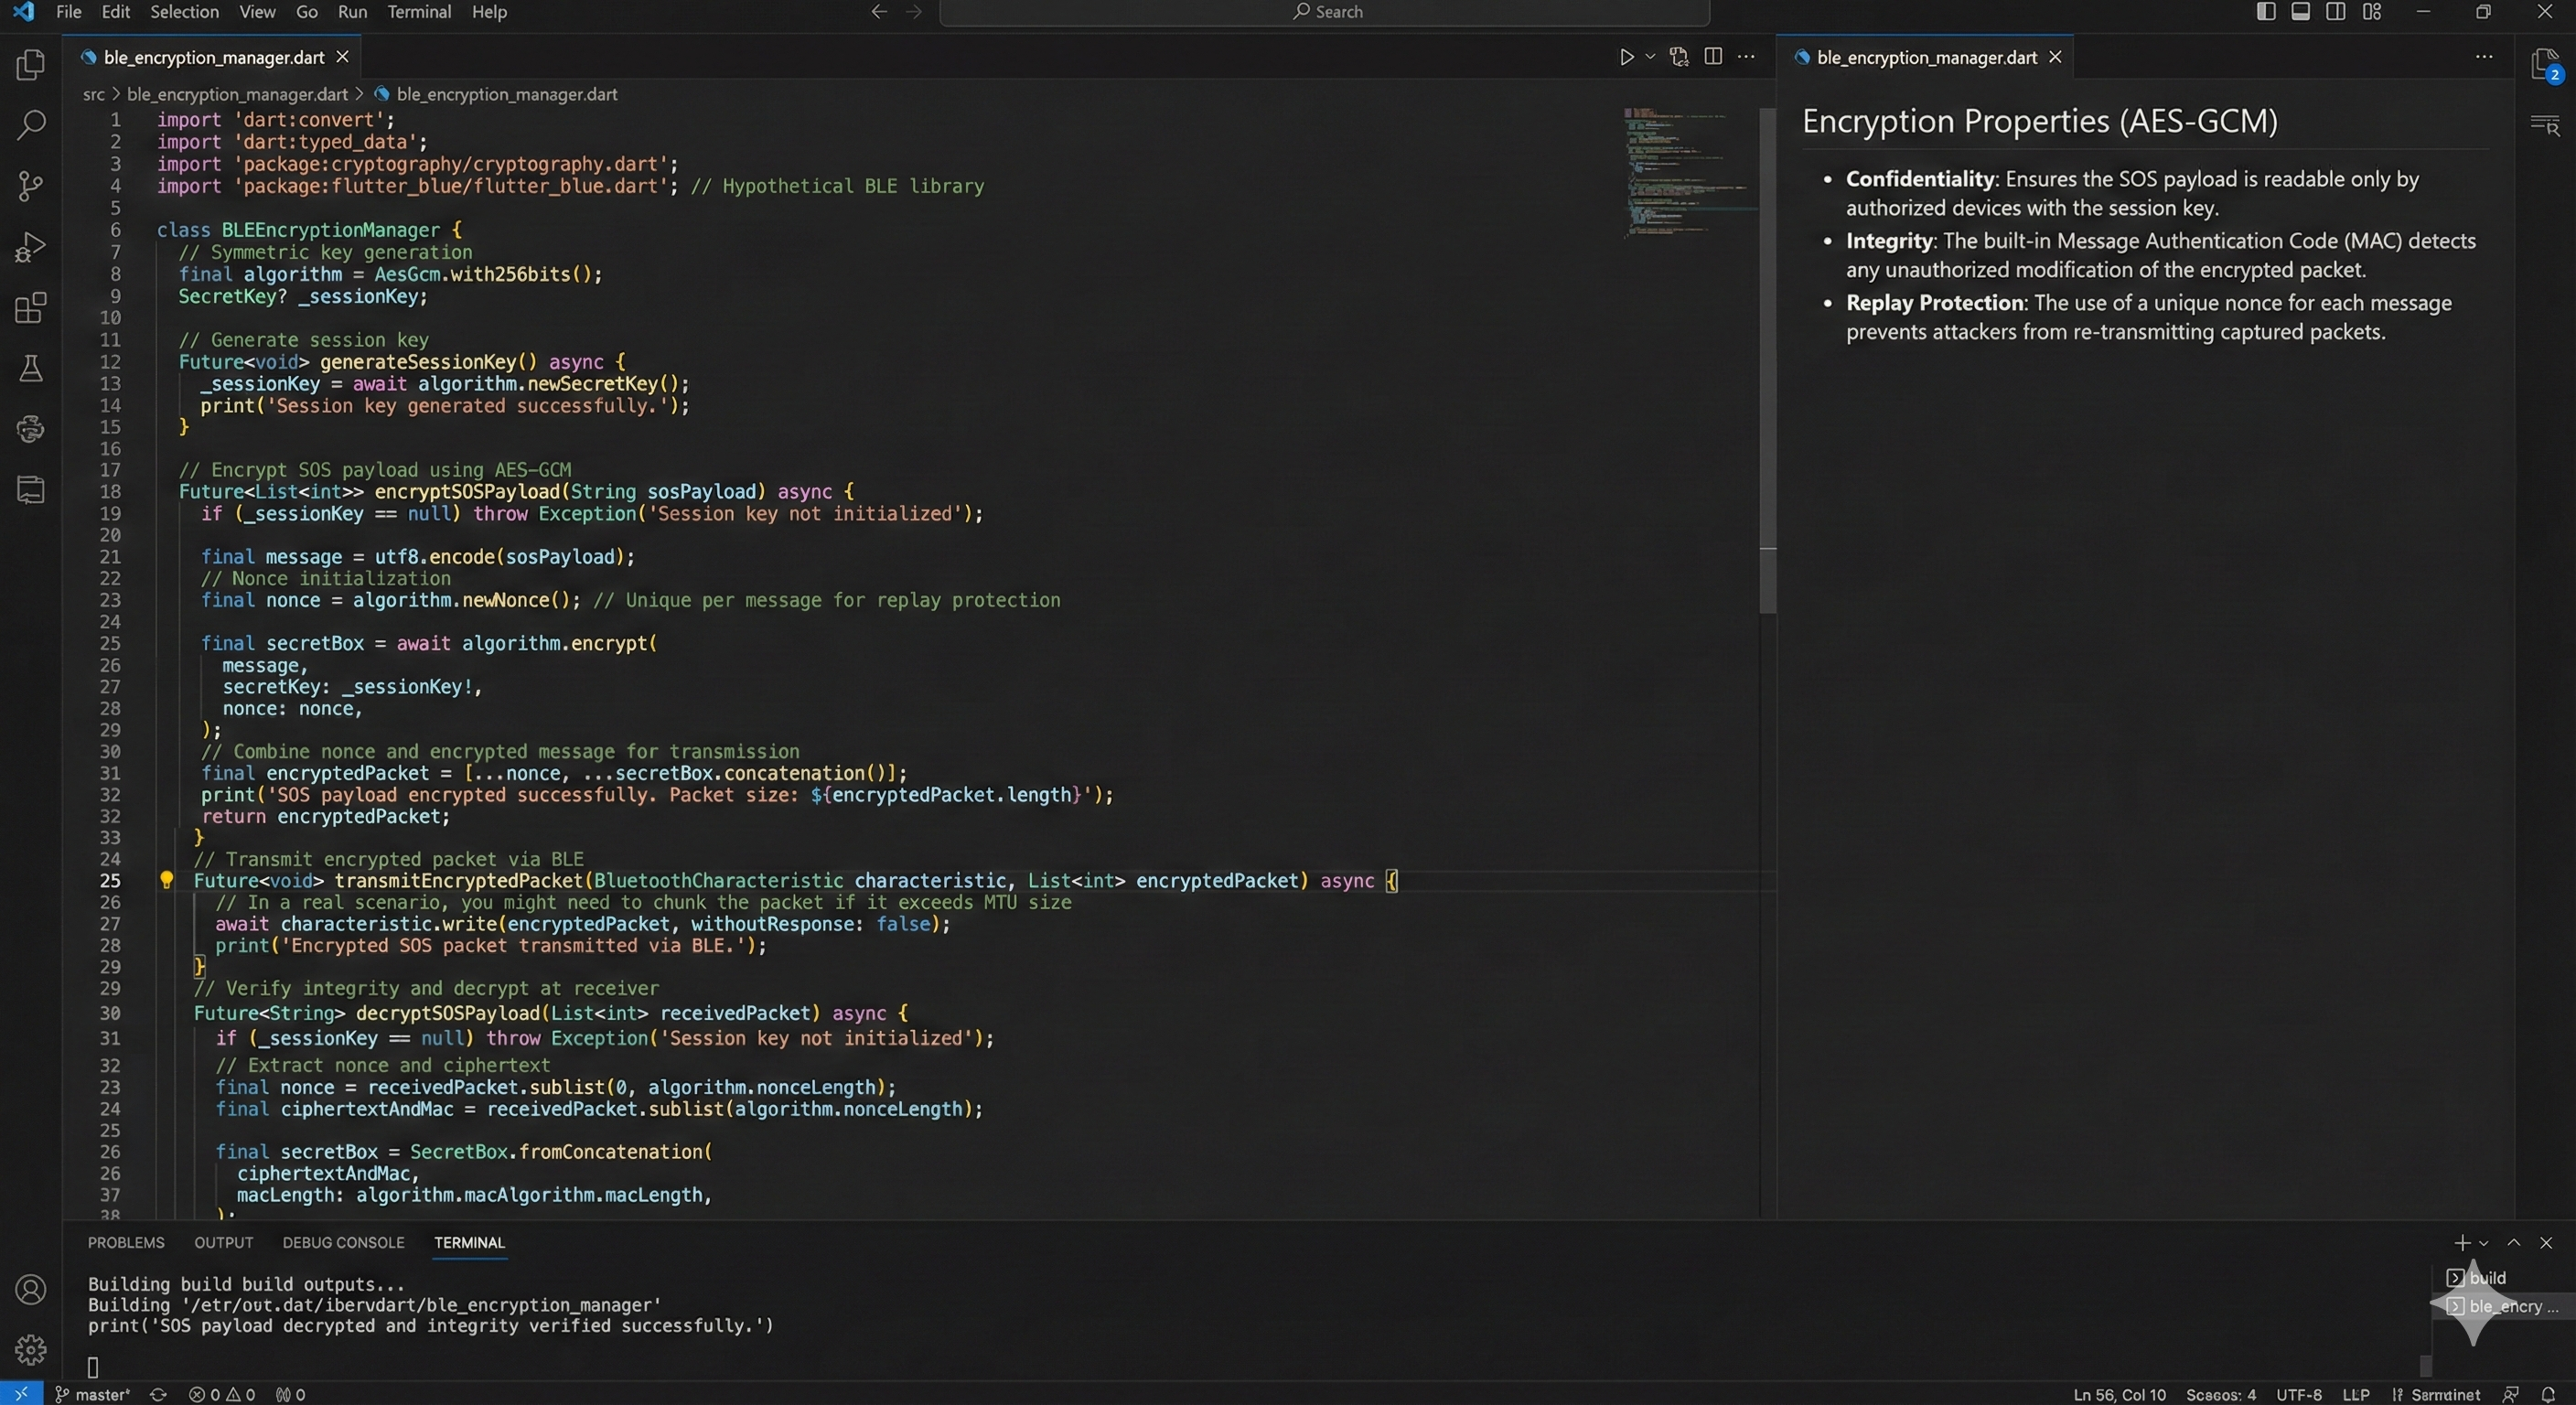
\includegraphics[width=0.85\textwidth]{chapters/ble_encryption_code.png}
    \caption{Encrypted BLE message transmission and reception implementation}
    \label{fig:ble_code}
\end{figure}

This implementation ensures both confidentiality and integrity of emergency data during offline peer-to-peer relay, preventing unauthorized access and tampering.

% -----------------------------------------------------------------------------
\section{AI-Based Emergency Classification Implementation}

Artificial Intelligence enables ResQNow to automatically analyze user inputs and prioritize emergency handling based on severity and type. The system employs a hybrid approach combining cloud-based AI for detailed analysis and rule-based logic for offline scenarios.

\subsection{AI Classification Pseudocode}

The following pseudocode outlines the AI-based emergency classification process:

\begin{algorithm}[H]
\caption{AI-Based Emergency Classification}
\begin{algorithmic}[1]
\State \textbf{Input:} User description of emergency (text or voice)
\State \textbf{Output:} Emergency type and severity level
\State
\Procedure{ClassifyEmergency}{$userInput$}
    \If{InternetAvailable()}
        \State $aiResponse \gets$ \Call{CloudAIClassification}{$userInput$}
        \State $emergencyType \gets$ \Call{ExtractType}{$aiResponse$}
        \State $severity \gets$ \Call{ExtractSeverity}{$aiResponse$}
        \State
        \If{$aiResponse.confidence < 0.7$}
            \State $severity \gets$ \Call{RuleBasedFallback}{$userInput$}
        \EndIf
    \Else
        \State $emergencyType \gets$ \Call{RuleBasedClassification}{$userInput$}
        \State $severity \gets$ \Call{RuleBasedSeverity}{$userInput$}
    \EndIf
    \State
    \State \Return \{type: $emergencyType$, severity: $severity$\}
\EndProcedure
\State
\Procedure{RuleBasedClassification}{$userInput$}
    \State $keywords \gets$ \Call{ExtractKeywords}{$userInput$}
    \State
    \If{"unconscious" OR "not breathing" in $keywords$}
        \State \Return \{type: "cardiac\_arrest", severity: "HIGH"\}
    \ElsIf{"bleeding" OR "blood" in $keywords$}
        \State \Return \{type: "severe\_bleeding", severity: "HIGH"\}
    \ElsIf{"burn" in $keywords$}
        \State \Return \{type: "burn\_injury", severity: "MODERATE"\}
    \ElsIf{"fracture" OR "broken" in $keywords$}
        \State \Return \{type: "fracture", severity: "MODERATE"\}
    \Else
        \State \Return \{type: "general\_emergency", severity: "LOW"\}
    \EndIf
\EndProcedure
\end{algorithmic}
\end{algorithm}

\subsection{Cloud-Based AI Classification Implementation}

The online AI module processes textual or voice-based user descriptions using cloud-based conversational AI services (OpenAI GPT or Google Gemini) to infer emergency context, extract symptoms, and determine severity level. Figure~\ref{fig:ai_online} shows the AI classification logic integrated with Firebase Firestore for persistent storage, including the API request structure, response parsing, confidence threshold checking, and database update operations.

\begin{figure}[H]
    \centering
    \includegraphics[width=0.95\textwidth]{chapters/ai_online_code.png}
    \caption{Cloud-based AI emergency classification and Firestore integration}
    \label{fig:ai_online}
\end{figure}

The implementation includes error handling for API failures and automatic fallback to rule-based classification when cloud services are unavailable or return low-confidence results.

\subsection{Offline AI Fallback Implementation}

To maintain functionality during connectivity loss or cloud service unavailability, ResQNow employs a rule-based fallback classification mechanism using keyword matching and predefined emergency patterns. Figure~\ref{fig:ai_offline} illustrates the offline AI decision logic, showing the keyword extraction process, severity mapping rules, and classification output structure used when cloud services are unavailable.

\begin{figure}[H]
    \centering
    \includegraphics[width=0.9\textwidth]{chapters/ai_offline_logic.png}
    \caption{Rule-based offline emergency classification logic}
    \label{fig:ai_offline}
\end{figure}

This hybrid approach ensures consistent emergency prioritization regardless of network conditions, maintaining system reliability during critical situations.

% -----------------------------------------------------------------------------
\section{Emergency Contact Notification Implementation}

The notification system ensures reliable alert delivery to emergency contacts through multiple redundant channels including push notifications, SMS, and email.

\subsection{Multi-Channel Notification Pseudocode}

The following pseudocode describes the multi-channel notification dispatch mechanism:

\begin{algorithm}[H]
\caption{Multi-Channel Emergency Notification}
\begin{algorithmic}[1]
\State \textbf{Input:} SOS alert data, emergency contact list
\State \textbf{Output:} Notifications sent via multiple channels
\State
\Procedure{NotifyEmergencyContacts}{$sosData$}
    \State $contacts \gets$ \Call{GetEmergencyContacts}{$sosData.userId$}
    \State $locationURL \gets$ \Call{GenerateMapURL}{$sosData.latitude$, $sosData.longitude$}
    \State
    \State $message \gets$ "Emergency Alert: " + $sosData.severity$ + 
    \State \hspace{2cm} " at " + $locationURL$
    \State
    \For{each $contact$ in $contacts$}
        \State // Send push notification
        \State \Call{SendPushNotification}{$contact.deviceToken$, $message$}
        \State
        \State // Send SMS
        \State \Call{SendSMS}{$contact.phoneNumber$, $message$}
        \State
        \State // Send Email
        \State \Call{SendEmail}{$contact.email$, "Emergency Alert", $message$}
    \EndFor
    \State
    \State \Call{LogNotificationStatus}{$sosData.id$, "notifications\_sent"}
\EndProcedure
\end{algorithmic}
\end{algorithm}

% -----------------------------------------------------------------------------
\section{Responder Acknowledgment Implementation}

The responder acknowledgment system enables nearby users to acknowledge emergency alerts and coordinate response efforts while preventing duplicate responses through atomic database transactions.

\subsection{Responder Acknowledgment Pseudocode}

The following pseudocode outlines the responder acknowledgment workflow:

\begin{algorithm}[H]
\caption{Responder Acknowledgment with Concurrency Control}
\begin{algorithmic}[1]
\State \textbf{Input:} SOS alert ID, responder user ID
\State \textbf{Output:} Acknowledgment status (success or already taken)
\State
\Procedure{AcknowledgeEmergency}{$sosId$, $responderId$}
    \State \Call{BeginTransaction}{}
    \State
    \State $sosAlert \gets$ \Call{GetSOSAlert}{$sosId$}
    \State
    \If{$sosAlert.responderId \neq null$}
        \State \Call{RollbackTransaction}{}
        \State \Return "Already acknowledged by another responder"
    \EndIf
    \State
    \State $sosAlert.responderId \gets$ $responderId$
    \State $sosAlert.responderName \gets$ \Call{GetUserName}{$responderId$}
    \State $sosAlert.responseTimestamp \gets$ \Call{GetCurrentTimestamp}{}
    \State $sosAlert.status \gets$ "ACKNOWLEDGED"
    \State
    \State \Call{UpdateSOSAlert}{$sosAlert$}
    \State \Call{CommitTransaction}{}
    \State
    \State \Call{NotifyOriginator}{$sosId$, $responderId$}
    \State
    \State \Return "Acknowledgment successful"
\EndProcedure
\end{algorithmic}
\end{algorithm}

% -----------------------------------------------------------------------------
\section{GPS Location Tracking Implementation}

Accurate location tracking is critical for emergency response coordination. The GPS module continuously monitors device location and provides real-time updates during active emergencies.

\subsection{Location Tracking Pseudocode}

The following pseudocode describes the GPS location tracking mechanism:

\begin{algorithm}[H]
\caption{Continuous GPS Location Tracking}
\begin{algorithmic}[1]
\State \textbf{Input:} Location permission granted
\State \textbf{Output:} Real-time GPS coordinates
\State
\Procedure{InitializeLocationTracking}{}
    \State \Call{RequestLocationPermission}{}
    \State
    \If{PermissionGranted()}
        \State \Call{StartLocationStream}{}
    \Else
        \State \Call{ShowPermissionError}{}
        \State \Return
    \EndIf
\EndProcedure
\State
\Procedure{OnLocationUpdate}{$location$}
    \State $latitude \gets$ $location.latitude$
    \State $longitude \gets$ $location.longitude$
    \State $accuracy \gets$ $location.accuracy$
    \State $timestamp \gets$ $location.timestamp$
    \State
    \If{EmergencyActive()}
        \State \Call{UpdateSOSLocation}{$latitude$, $longitude$, $timestamp$}
        \State \Call{NotifyContactsOfLocationUpdate}{$latitude$, $longitude$}
    \EndIf
    \State
    \State \Call{CacheLocation}{$latitude$, $longitude$} // For offline use
\EndProcedure
\end{algorithmic}
\end{algorithm}

% -----------------------------------------------------------------------------
\section{Database Schema and Data Models}

The system uses Firebase Firestore as the primary database with the following collection structure and data models.

\subsection{Firestore Data Structure}

The database schema is organized into the following collections:

\begin{itemize}
    \item \textbf{users/\{userId\}} - User profile information
    \begin{itemize}
        \item Fields: name, email, phone, bloodGroup, medicalNotes
        \item Subcollection: contacts/\{contactId\} - Emergency contacts
    \end{itemize}
    
    \item \textbf{sos\_alerts/\{sosId\}} - Emergency alert records
    \begin{itemize}
        \item Fields: userId, latitude, longitude, timestamp, severity, type, status
        \item Fields: responderId, responderName, responseTimestamp
    \end{itemize}
    
    \item \textbf{ble\_queue/\{messageId\}} - Queued offline messages
    \begin{itemize}
        \item Fields: encryptedData, hopCount, originDeviceId, timestamp
    \end{itemize}
\end{itemize}

% -----------------------------------------------------------------------------
\section{Summary}

This chapter presented the complete implementation of the ResQNow emergency response system through detailed pseudocode and code implementations. It demonstrated SOS activation logic, BLE-based offline communication with encryption, AI-driven emergency classification with online and offline support, multi-channel notification dispatch, responder acknowledgment with concurrency control, and GPS location tracking. The presented pseudocode and code-level evidence confirms the technical feasibility, robustness, and real-world readiness of the proposed system.

}